\documentclass[10pt,a4paper]{article}
\usepackage[top=3cm,bottom=3cm,includeheadfoot]{geometry}	% Seitengeometrie festlegen
\usepackage[ngerman]{babel}
\usepackage{fancyhdr}						% das nötige Paket um Fuß- / Kopfzeilen zu verwenden			
\usepackage[utf8]{inputenc}
\usepackage{amsmath}
\usepackage{amsfonts}
\usepackage{amssymb}
\usepackage{caption}
\usepackage{listings}
\usepackage{textcomp}
\usepackage{graphicx}
\usepackage{color}
\newcommand{\hilight}[1]{\colorbox{yellow}{#1}}
\usepackage{chngcntr}
\usepackage{hyperref}
\usepackage{caption}
\usepackage{colortbl}

\counterwithin{figure}{section}

\author{Ken Hasenbank, Artur Schmidt}
\title{Praktikum 3}
\date{24.01.2018}

\makeatletter

\pagestyle{fancy}	%ermöglicht die Verwendung von eigens bearbeiteten Kopf-/ Fußzeilen
\fancyhf{}
%Bearbeiten der Kopzeile
\fancyhead[R]{\thepage}
\fancyhead[C]{Chaos \& Fraktale}
\fancyhead[L]{\@date}
\renewcommand{\headrulewidth}{0.4pt} %obere Trennlinie
%Bearbeiten der Fußzeile
\fancyfoot[C]{ \centering Ken Hasenbank,\linebreak Artur Schmidt}
\renewcommand{\footrulewidth}{0.4pt} %untere Trennlinie


\begin{document}
%\thispagestyle{empty}		% legt ein für diese Seite ein Layout fest, dass leer ist (keine Fuß-/ Kopfzeile etc) 

%%%%%%%%%%%%  DECKBLATT ANFANG   %%%%%%%%%%%%%%
\begin{titlepage}
\begin{center}
	\Large{Hochschule Darmstadt}\\
	\large{Fachbereich Informatik}
\end{center}

\vspace{1cm}
\begin{center}
	\large{Chaos und Fraktale}
\end{center}

\vspace{2,5cm}
\begin{center}
	\huge{Praktikum}\\
\end{center}

%\begin{center}
%	\Huge{\textbf{Praktikum 1}} 
%\end{center}


\vspace{6cm}
\begin{center}
{\large 
\begin{tabular}{lll}
	Semester: && SoSe 2017\\
	\vspace{1mm}\\
	Laboranten: && Ken Hasenbank\\
	&& Artur Schmidt\\
	\vspace{1 mm}\\
	Datum:	&& \@date\\
	\end{tabular} 
	}%\large beenden
\end{center}

\end{titlepage}
%%%%%%%%%%%%  DECKBLATT ENDE  %%%%%%%%%%%%%%5

\section{Punkt 1}
Definieren wir ein L-System mit:
\begin{lstlisting}
Axiom: F
Adjustment Angle: 90
Produktion: F>FF+F|F+FF
\end{lstlisting}

Erhalten wir folgendes Fraktal:
\begin{center}
	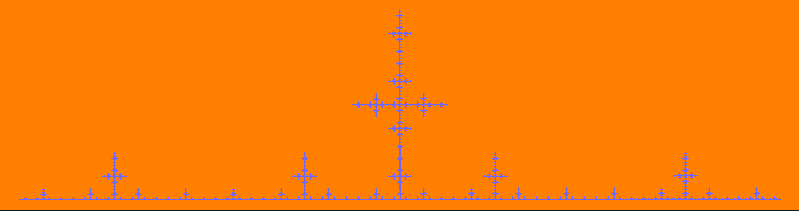
\includegraphics[scale=0.5]{images/lin.PNG}
	\captionof{figure}{L-System Fraktal}
\end{center}


\end{document}
\makeatother